% ------------------------------------------------------------------------------ %
% The ?rst information LATEX needs to know when processing an input ?le is
% the type of document the author wants to create. This is speci?ed with the
% \documentclass command.
%
%   \documentclass[options]{class}
%
% Here class speci?es the type of document to be created.

\documentclass[a4paper,11pt]{article}

% The above command instructs LATEX to typeset the document as an article with
% a base font size of eleven points, printing on A4 paper.
% ------------------------------------------------------------------------------- %


% ------------------------------------------------------------------------------- %
% While writing your document, you will probably ?nd that there are some
% areas where basic LATEX cannot solve your problem. If you want to include
% graphics, coloured text or source code from a ?le into your document, you
% need to enhance the capabilities of LATEX. Such enhancements are called
% packages. Packages are activated with the
%
%   \usepackage[options]{package}
%
% command, where package is the name of the package and options is a list of
% keywords that trigger special features in the package.
%
% ATTENTION: IN ORDER TO ENABLE THE GREEK TYPESETTING YOU NEED TO INCLUDE IN YOUR
%            PREAMBLE SPECIFIC PACKAGES VIA THE USE OF THE \usepackage COMMAND.
%
%            THE SAME IS TRUE FOR SPECIFIC MATH FONTS ETC.


% * Activating Greek fonts in Latex
  \usepackage[english,greek]{babel} % the last language is the default

  %% > UNCOMMENT if your editor uses iso-8859-7 encoding for Greek (typical in Windows System).
  %\usepackage[iso-8859-7]{inputenc}

  %% > UNCOMMENT if your editor uses Unicode encoding for Greek (typical in POSIX Systems).
  \usepackage[utf8x]{inputenc}

  % One bad thing about the babel package is that it cannot discriminate explicitly between
  % Greek and Latin fonts, so you have to state commands in order to signify where the
  % Latin charecters begin and where they end and the Greek characters begin. For this
  % job the \latintext and \greektext commands exist. However Latex give you the versatility
  % to create wildcards for all of each commands and thus, to create alias with shorter
  % word length. Below we create the aliaces \lt and \gt for the \textlatin and \textgreek
  % commands respectively.

  \newcommand{\lt}{\latintext}
  \newcommand{\gt}{\greektext}


% * Math packages
 % \usepackage{amsthm}
  \usepackage{amsmath}
 % \usepackage{amssymb}

% * graphics package
  \usepackage[pdftex]{graphicx} % remove the 'pdftex' option if not PDFLatex is used.

% * verbatim writing package (mainly used to import program's code)
  \usepackage{verbatim}

% ------------------------------------------------------------------------------- %


% ------------------------------------------------------------------------------- %
% Here we set the title, the author and the date of our document.
%
% * Setting the title of the document
  \title{1η Υποχρεωτική Εργασία\\
Στο Μάθημα της Αριθμητικής Ανάλυσης} % Put your own title here

% * Setting the author or authors of the document
  \author{Όνοματεπώνυμο: Γεώργιος Δάλλας  \\  ΑΕΜ: 4116}       % Put your own Name and AEM here

% * Setting the date of the document
  \date{\today}                                      % Put a specific date here
% ------------------------------------------------------------------------------- %


% =============================================================================== %
% ||                       HERE WE BEGIN OUR DOCUMENT                          || %
% =============================================================================== %
\begin{document}

% *** We are now inside the document everything from now on is VISIBLE!!! *** %

% Command that prints the title of your document
\maketitle

\section{Πρώτη Άσκηση}

\begin{center}
    Γραφική παράσταση της $f(x)=\mathrm{e}^{\sin^3\left(x\right)}+x^6-2x^4-x^3-1$.
    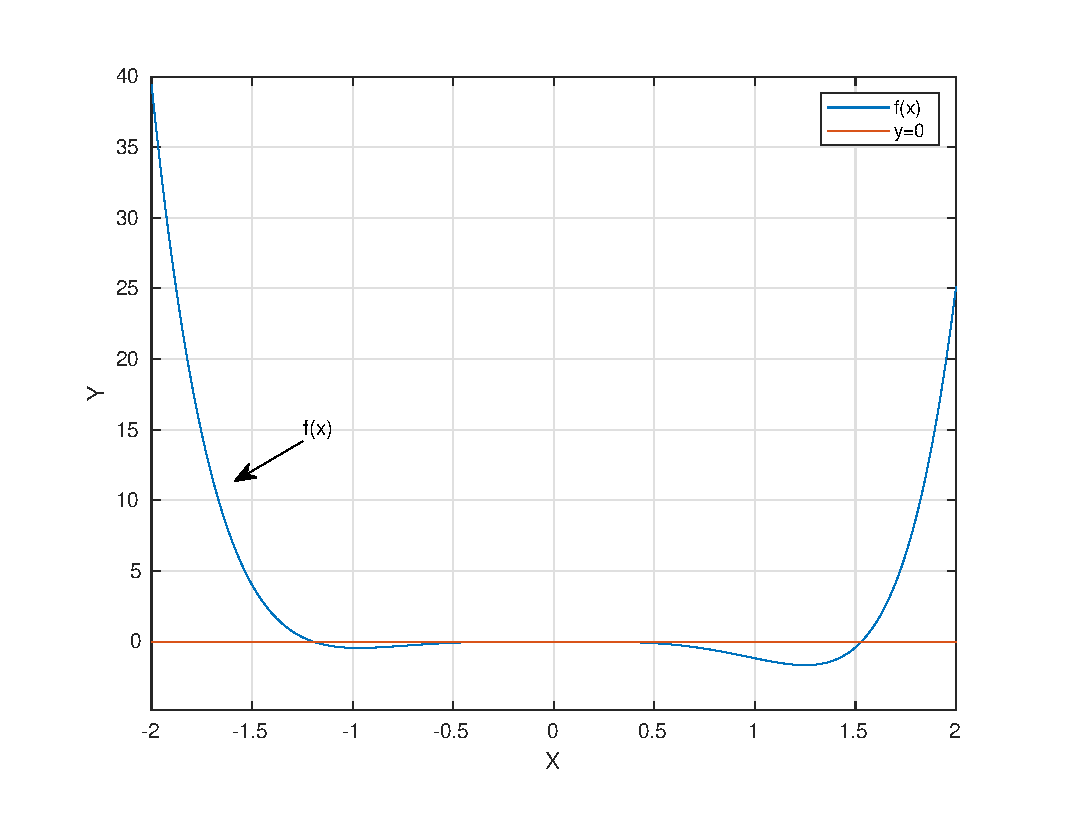
\includegraphics[width=12cm]{ask1.eps}\\
\end{center}
\newpage
    Μετά απο την εφαρμογή των μεθόδων διχοτόμησης, \lt Newton-Raphson \gt και τέμνουσας στην συνάρτηση $f(x)=\mathrm{e}^{\sin^3\left(x\right)}+x^6-2x^4-x^3-1$,  οι 3 ρίζες που βρέθηκαν είναι οι εξής:
    \begin{enumerate}
        \item $x_{1}=-1.19762$
        \item $x_{2}=0$
        \item $x_{3}=1.53013$
    \end{enumerate}
   Τα διαστήματα που χρησιμοποιήθηκαν για την εύρεση της κάθε ρίζας είναι τα εξής:
   \begin{enumerate}
        \item $x_{1}:[-2,-1]$
        \item $x_{2}:[-1,1]$
        \item $x_{3}:[\frac{13}{10},2]$
    \end{enumerate}
	\par
 Για την ρίζα $x_{1}$, στην μέθοδο διχοτόμησης, χρειάστηκαν 18 επαναλήψεις
 για την επίτευξη της ακρίβειας 5 δεκαδικών ψηφίων. Για την μέθοδο \lt 
 Newton-Raphson \gt χρησιμοποιήθηκαν 9 επαναλήψεις και για την μέθοδο 
 τέμνουσας 14. Το αποτέλεσμα είναι αναμενόμενο, καθώς η μέθοδος \lt Newton-
 Raphson \gt θεωρείται γρηγορότερη με την μέθοδο της τέμνουσας να ακολουθεί.
 Η μέθοδος της διχοτόμησης είναι αργή αλλά αξιόπιστη.
 \par 
    Για την χρήση της μεθόδου διχοτόμησης, η συνάρτηση θα πρέπει να είναι
    συνεχής και τα άκρα του διαστήματος που χρησιμοποιούνται να είναι 
    αντίθετου προσήμου. Δυστηχώς, για την ρίζα $x_{2}=0$, δεν είναι δυνατή η
    εύρεση ενός τέτοιου διαστήματος, οπότε η χρήση της μεθόδου διχοτόμησης
    καθίσταται αδύνατη. Ακόμη, για $x=0$ η 
$f'(x)=3\mathrm{e}^{\sin^3\left(x\right)}\cos\left(x\right)\sin^2\left(x\right)+6x^5-8x^3-3x^2$ 
ισούται με 0, άρα ενώ στις υπόλοιπες τετραγωνικές ρίζες
($f'(x_{1}),f'(x_{2}) \neq 0$) η μέθοδος \lt Newton-Raphson \gt είναι η πιο
αποδοτική, στην συγκεκριμένη ρίζα, καταφέρνει και φτάνει σε μια 
ικανοποιητική προσέγγιση μετά απο 32 επαναλήψεις. Αυτό παρατηρείται γενικά
σαν πρόβλημα με τις ρίζες που δεν συγκλίνουν τετραγωνικά στην μέθοδο αυτή. 
Η συμπεριφορά αυτή μπορεί να εξηγηθεί εύκολα, καθώς με την μέθοδο του \lt Newton-
Raphson \gt, χρησιμοποιείται εφαπτομένη της κάθε προσέγγισης στη συνάρτηση,
για να βρεθεί η επόμενη προσέγγιση. Άρα με παράγωγο 0, η εφαπτομένη προφανώς
θα οδηγήσει σε μια πολύ πιο μακρινή προσέγγιση από την επιθυμητή.. Επίσης προβληματική είναι και η μέθοδος της 
τέμνουσας, καθώς όταν $f'=0$, μπορεί να χαλάσει η σύγκλιση του αλγορίθμου.
Οπότε και με την μέθοδο της τέμνουσας, η μέθοδος καταλήγει σε μια κοντινή
προσέγγιση έπειτα από 53 επαναλήψεις. \par
    Τέλος, για την ρίζα $x_{3}$, η μέθοδος της διχοτόμησης χρειάστηκε 18 
    επαναλήψεις, η μέθοδος \lt Newton-Raphson  \gt 8 και η μέθοδος της 
    τέμνουσας 10, που είναι παρόμοια αποτελέσματα με την πρώτη ρίζα και 
    αναμενόμενα, γνωρίζοντας την αποδοτικότητα των παραπάνω μεθόδων.
    
    
\section{Δεύτερη Άσκηση}
\begin{center}
    Γραφική παράσταση της\\ $f(x)=
    94cos(x)^3-24*cos(x)+177sin(x)^2-108*sin(x)^4-72*cos(x)^3sin(x)^2-65$.
    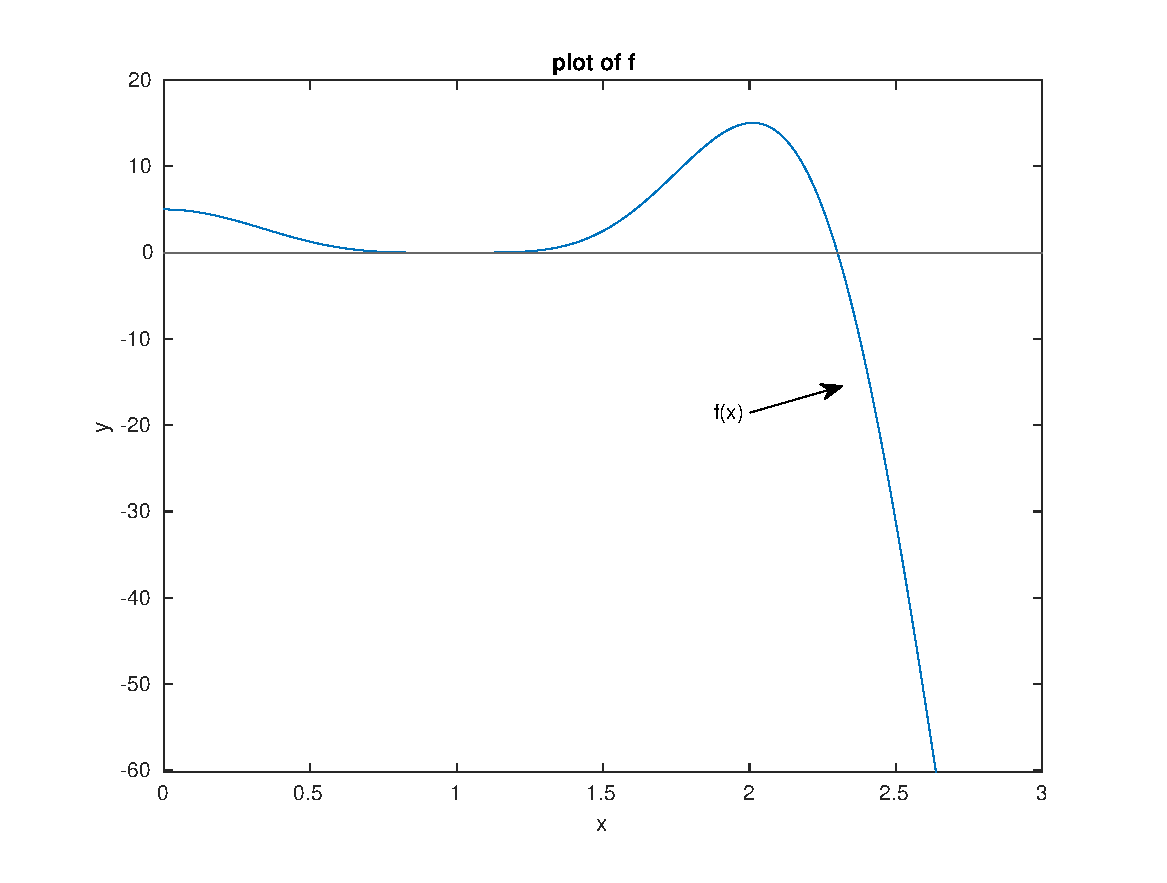
\includegraphics[width=12cm]{ask2.eps}\\
\end{center}

    Μετά απο την εφαρμογή των τροποποιημένων μεθόδων διχοτόμησης, \lt Newton-Raphson
    \gt και τέμνουσας στην συνάρτηση $f(x)=94cos(x)^3-24*cos(x)+177sin(x)^2-
    108*sin(x)^4-72*cos(x)^3sin(x)^2-65$,  οι 3 ρίζες που βρέθηκαν είναι οι εξής:
    \begin{enumerate}
        \item $x_{1}=0.84106$
        \item $x_{2}=1.04720$
        \item $x_{3}=2.30052$
    \end{enumerate}
   Τα διαστήματα που χρησιμοποιήθηκαν για την εύρεση της κάθε ρίζας είναι τα
   εξής:
   \begin{enumerate}
        \item $x_{1}:[0,\frac{7}{8}]$ 
        \item $x_{2}:[\frac{9}{10},2]$
        \item $x_{3}:[\frac{21}{10},3]$
    \end{enumerate}
    \newpage
Για την τροποποιημένη μέθοδο τέμνουσας το τρίτο σημείο που χρησιμοποιήθηκε 
σε κάθε διάστημα, είναι το μέσο του διαστήματος αυτού.
Μετά από την εκτέλεση του τροποποιημένου αλγορίθμου διχοτόμησης 10 φορές, 
καταγράφηκαν τα εξής αποτελέσματα για της επαναλήψεις που χρειάστηκαν στην
εύρεση της ρίζας:
\begin{center}
\begin{tabular}{ |c|c|c| } 
 \hline
 $x_{1}$ & $x_{2}$ & $x_{3}$ \\ 
 \hline
 18 & 23 & 18 \\ 
 27 & 24 & 29 \\ 
 26 & 25 & 24 \\ 
 14 & 21 & 30 \\ 
 29 & 21 & 25 \\ 
 27 & 37 & 24 \\ 
 20 & 25 & 32 \\ 
 29 & 20 & 30 \\ 
 22 & 20 & 22 \\ 
 24 & 20 & 28 \\ 
 \hline
\end{tabular}
\end{center} 
Όπως εύκολα παρατηρείται, ο αλγόριθμος δεν συγκλίνει πάντα στο ίδιο σημείο.
Το χαρακτηριστικό αυτό οφείλεται στο γεγονός ότι στον καθορισμό του επόμενου 
διαστήματος που χρησιμοποιείται σε κάθε επανάληψη, επιλέγεται πάντα 
ένα τυχαίο σημείο που ανήκει στο προηγούμενο διάστημα.
\par
Για την σύγκριση ταχύτητας σύγκλισης των τροποποιημένων με των κλασικών 
μεθόδων, χρησιμοποιήθηκαν 1000 τυχαία διανύσματα. Έπειτα από την καταγραφή 
των αποτελεσμάτων, συμπεραίνεται ότι η τροποποιημένη μέθοδος διχοτόμησης 
είναι 35.04\% πιο αργή από την 
κλασική. Η τροποποιημένη μέθοδος τέμνουσας είναι 35.73\% πιο αργή και η 
τροποποιημένη μέθοδος Newton-Raphson 59.9\% πιο γρήγορη. \\
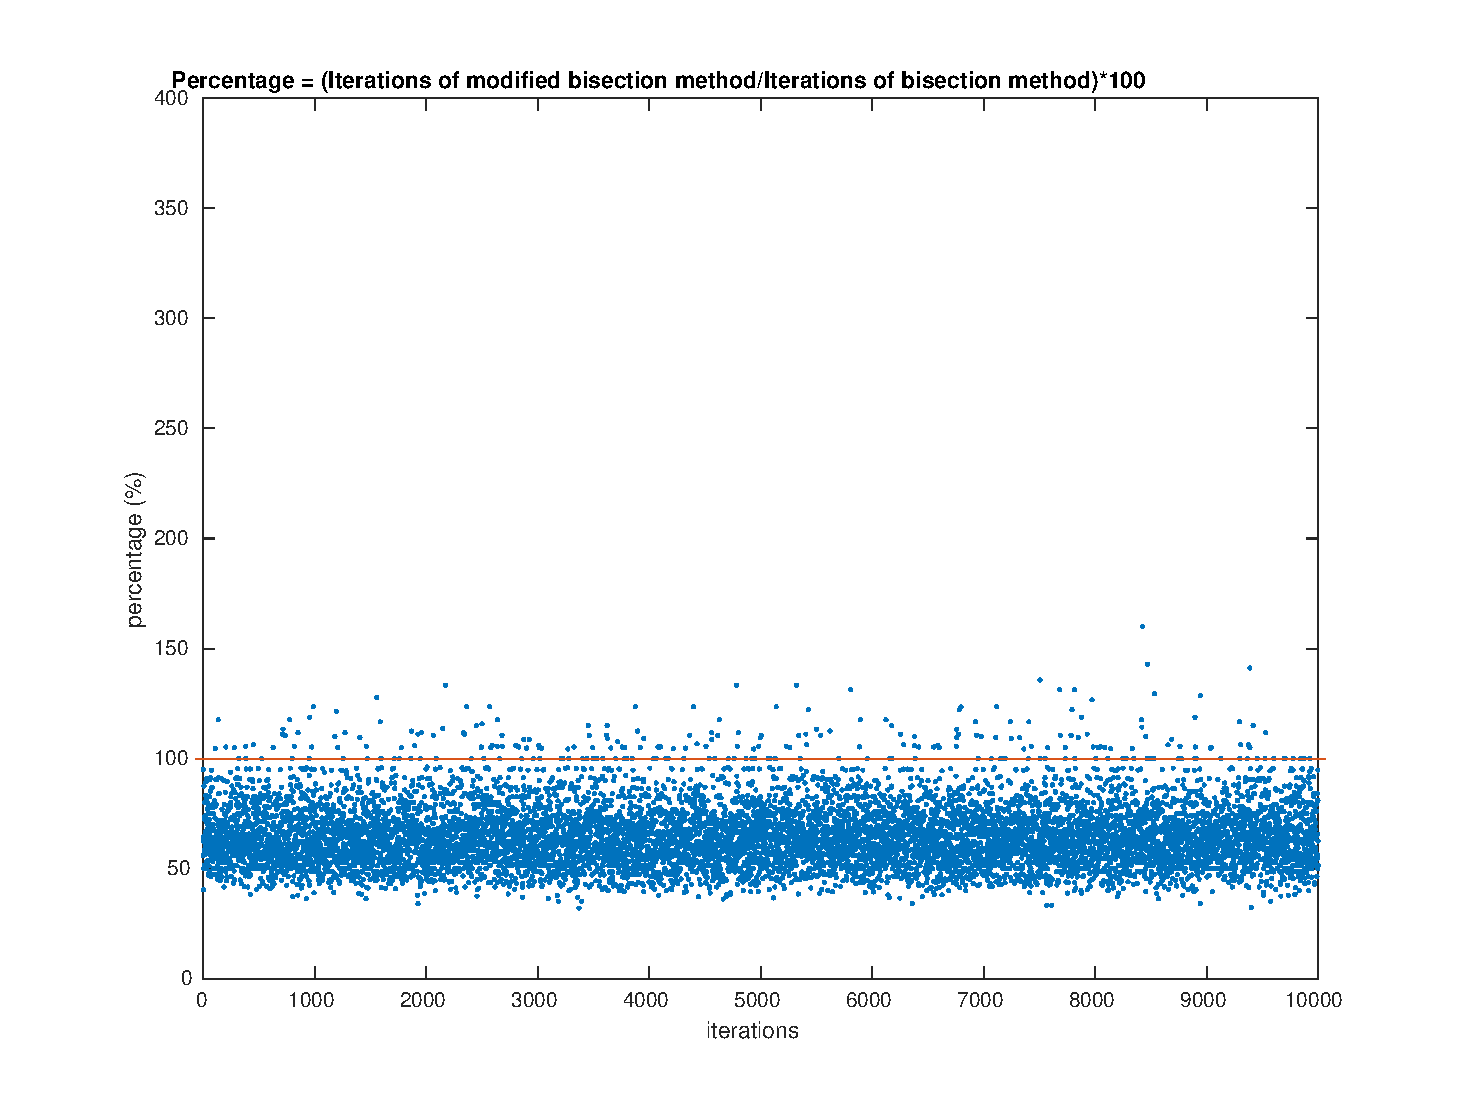
\includegraphics[width=12cm]{stat1.eps}\\
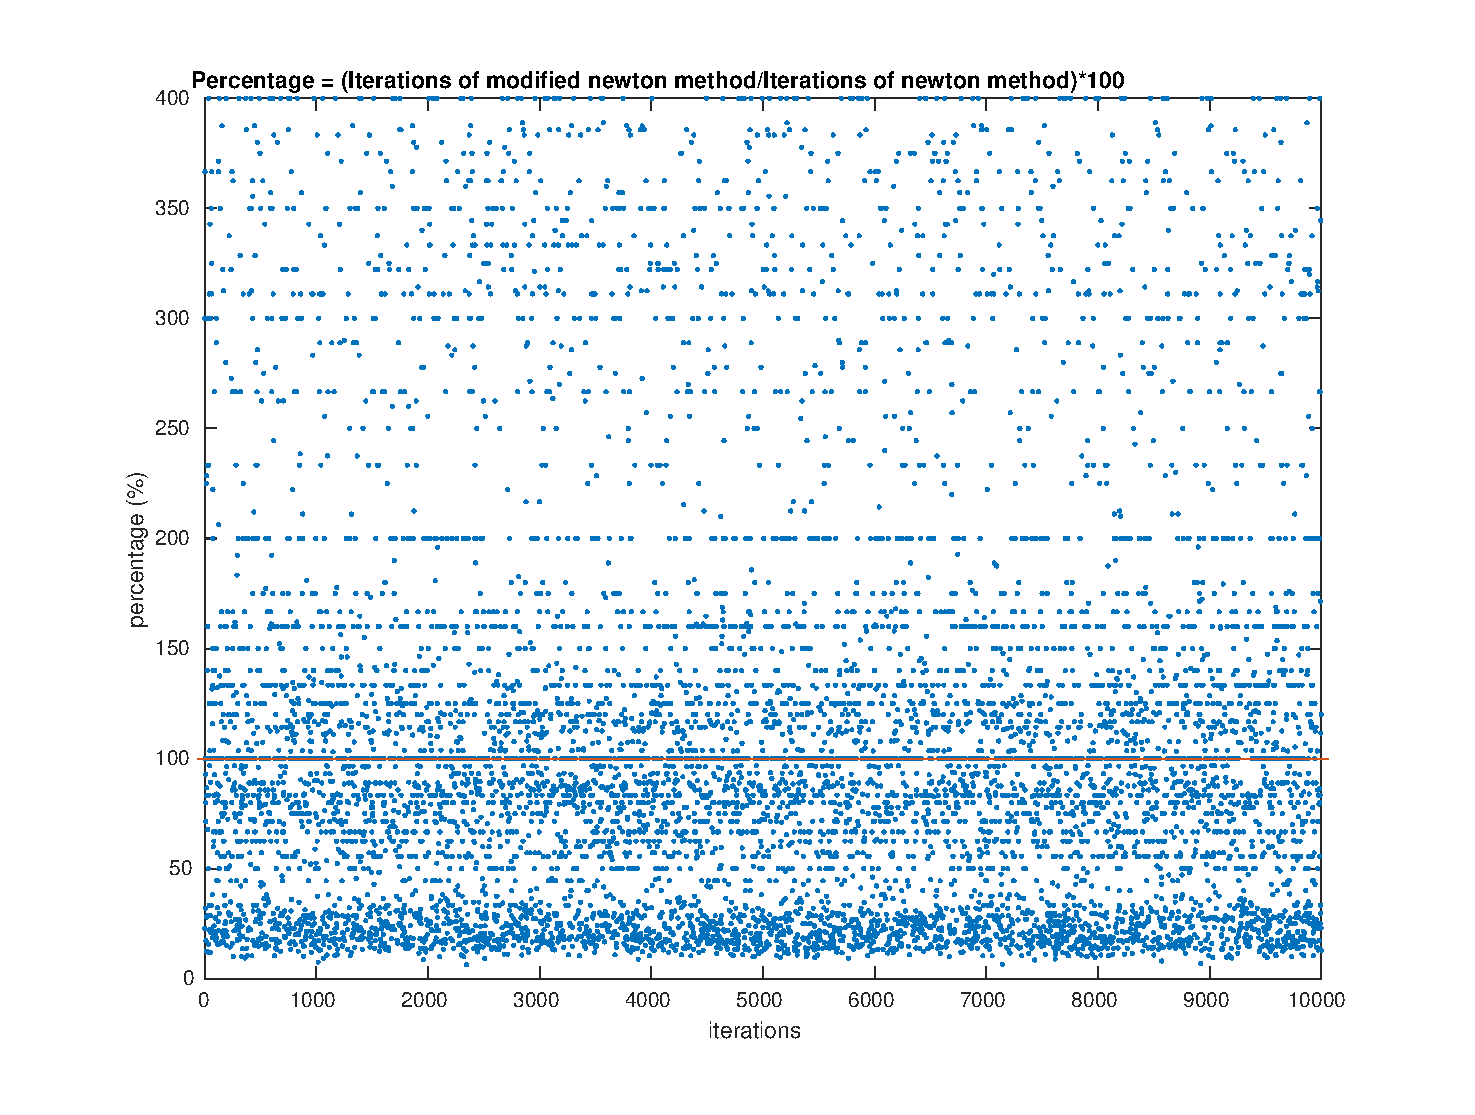
\includegraphics[width=12cm]{stat2.eps}\\
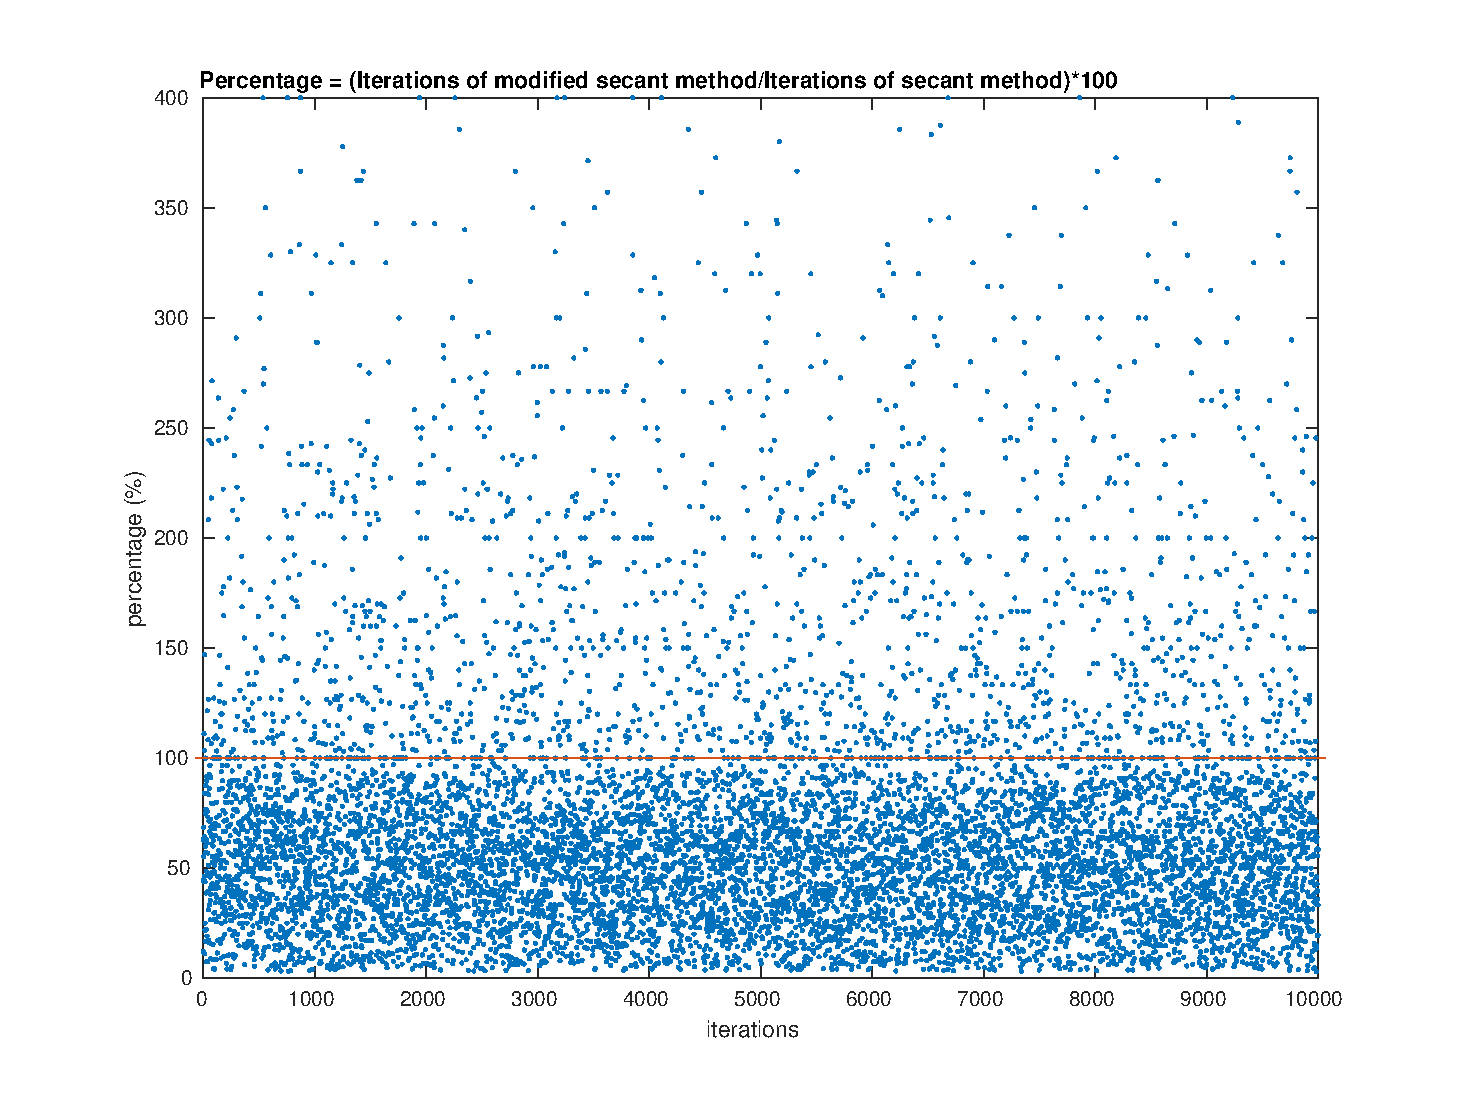
\includegraphics[width=12cm]{stat3.eps}\\

\section{Τρίτη Άσκηση}
Για την παραγοντοποίηση \lt PA=LU \gt ζητείται ενας πίνακας Α και ένα δυάνισμα \lt 
b\gt. Ο πίνακας Α που χρησιμοποιήθηκε είναι ο εξής: \\
$Α=\begin{bmatrix}
5 & 2 & 2\\
4 & 6 & 4\\
4 & 2 & 2
\end{bmatrix}$ \\
To δυάνισμα \lt b \gt που χρησημοποιήιηκε είναι το παρακάτω: \\
$b=\begin{bmatrix}
4 \\
-6 \\
7 
\end{bmatrix}$ \\
To διάνυσμα αγνώστων \lt x \gt που παρήγαγε η συνάρτηση έχει τις εξής τιμές:
$x=\begin{bmatrix}
-3 \\
-16 \\
25.5
\end{bmatrix}$ \\
Ελέγχοντας τις τιμές, λύνεται το παραπάνω γραμμικό σύστημα, επιβεβαιώνοντας
έτσι ότι η συνάρτηση λειτουργεί σωστά.
\par
Για την συνάρτηση \lt Cholesky \gt, αρχικά γράφτηκε ένας έλεγχος για τον 
πίνακα εισόδου, καθώς η μέθοδος λειτουργεί μόνο για θετικά ορισμένους συμμετρικούς πίνακες.
\newpage Για είσοδο στην συνάρτηση εισάγεται ο παρακάτω πίνακας:\\
\begin{center}
$MatrixForCholesky=\begin{bmatrix}
4 & 12 & -16\\
12 & 37 & -43\\
-16 & -43 & 98
\end{bmatrix}$ \\
\end{center}
και η έξοδος που παράγει είναι ο κάτω τριγωνικός πίνακας \\
\begin{center}
$L=\begin{bmatrix}
2 & 0 & 0\\
6 & 1 & 0\\
-8 & 5 & 3
\end{bmatrix}$
\end{center}
όπου είναι και το αναμενόμενο αποτέλεσμα, επιβεβαιώνοντας την ορθή 
λειτουργία της συνάρτησης. \par
Για την μέθοδο Gauss-Seidel, αρχικά δημιουργείται ένας $nxn$ μηδενικός 
πίνακας στην συνάρτηση \lt GaussSeidelMakeMatrix(n) \gt και στην συνέχεια
αλλάζουν συγκεκριμένες τιμές του πίνακα για την δημιουργία του απαιτούμενου
αραιού συστήματος. Η ίδια συνάρτηση εκτός από τον πίνακα Α που απαιτείται 
για την λύση του συστήματος επιστρέφει και το διάνυσμα \lt b 
\gt. Στο πρόγραμμα εμφανίζεται η λύση του συστήματος για $n=10$ αλλά καθώς 
για $n=10000$, παράγονται 10000 λύσεις, για τον έλεγχο των τιμών απαιτείται
η προβολή του πίνακα \lt x \gt στο \lt workspace \gt του \lt Matlab \gt μετά 
την εκτέλεση του προγράμματος.\\


\section{Τέταρτη Άσκηση}


Για την στοχαστικότητα του πίνακα \lt G \gt, αρκεί είτε το άθροισμα κάθε γραμμής είτε
στήλης του πίνακα να ισούται με 1. Μετά από αυτόν τον έλεγχο στο πρόγραμμα 
εμφανίζει ότι ο πίνακας είναι δεξιά στοχαστικός, άρα το ότι το άθροισμα κάθε στήλης 
είναι ίσο με 1. \par
Προφανώς για την απόδειξη της στοχαστικότητας έχει δημιουργηθεί ήδη ο πίνακας \lt G 
\gt και μετά των υπολογισμό του ιδιοδιανύσματος της μέγιστης ιδιοτιμής με την μέθοδο
της δυνάμεως και εμφανίζοντας το στην οθόνη ως \lt p \gt, επιβεβαιώνεται ότι είναι 
ίδιο με αυτό της εκφώνησης. \par
Για το ερώτημα 3, η σύνδεση που αφαιρέθηκε είναι από τον κόμβο 13 στον 14. Στην 
συνέχεια προστέθηκαν συνδέσεις από τον 13 στον 10, από τον 11 στον 10, από τον 8 
στον 10 και από τον 15 στον 10. Εν τέλει, ο βαθμός σημαντικότητας του κόμβου 10 από 
0.106320 αυξήθηκε σε 0.243154 και έγινε ο μεγαλύτερος από όλους.
\par
Η αλλαγή του \lt q \gt σε 0.02, φαίνεται να μειώνει τον βαθμό σημαντικότητας των σελίδων που κατατάσσονται 
χαμηλά και να αυξάνει την σημαντικότητα των δημοφιλέστερων σελίδων αντίστοιχα. Η αλλαγή του \lt q \gt σε 0.6, εξισορροπεί τις τιμές, καθώς αυξάνεται η τυχαιότητα, με 
αποτέλεσμα την αύξηση του βαθμού σημαντικότητας μη δημοφιλών σελίδων και την μείωση
των υψηλά κατατασσόμενων αντίστοιχα. Η πιθανότητα μεταπήδησης είναι αναγκαία καθώς μπορεί όλες οι σελίδες να μην είναι συνδεδεμένες μεταξύ τους. Έτσι ο αλγόριθμος δεν θα υπολογίσει ποτέ τον βαθμό σημαντικότητας των σελίδων που δεν είναι συνδεδεμένες με τις υπόλοιπες. \par
Aντικαθιστώντας το A(8,11) και το A(12,11) με 3 στον πίνακα γειτνίασης, πετυχαίνεται ο
στόχος βελτίωσης του βαθμού σημαντικότητας της σελίδας 11, αλλά όχι τόσο
αποτελεσματικά. Αυτό συμβαίνει λόγω της συνδεσιμότητας που υπάρχει με την σελίδα
11, με αποτέλεσμα να μεταφέρεται η σημαντικότητα και να μοιράζεται σε άλλους κόμβους
όπως την σελίδα 15, που παρουσιάζει σχεδόν την ίδια αύξηση με την σελίδα 11. \par
Η αφαίρεση του κόμβου 10, έχει ως αναμενόμενο αποτέλεσμα, την αύξηση της 
τάξης των σελίδων 1,2,3,4,5,6,7,8,11. Η τάξη των υπόλοιπων σελίδων 
μειώνεται. Η μεγαλύτερη αύξηση παρατηρείται στην σελίδα 11. Αυτό είναι 
λογικό καθώς οι σελίδες  6,7 και 14 που συνδεόταν και με την σελίδα 10 και 
με την 11, πλέον έχουν μια σύνδεση λιγότερη, αυξάνοντας την σημαντικότητα 
της σύνδεσης αυτής. Η μεγαλύτερη μείωση τάξης που παρατηρείται είναι για την
σελίδα 13. Προηγουμένως, η μοναδική σύνδεση που είχε η σελίδα 10 προς μια 
άλλη σελίδα ήταν η 13, οπότε με την αφαίρεση της σελίδας 10, χάνεται αυτό το 
σημαντικό κομμάτι της τάξης της σελίδας 13.




% =============================================================================== %
% ||                       HERE WE END OUR DOCUMENT                          || %
% =============================================================================== %
\end{document}